\subsection{Structure du second étage}
\label{subsec:second_etage}

\subsubsection{Flèche}
\label{subsubsec:second_etage}
Pour le tube du second étage de 80mm interne et 2mm d'épaisseur, nous avons mesuré une petite flèche sur deux côtés opposés mais assez négligeable.\\
Le test dynamique sera réalisé dès que possible.
vsgdhvvdsqgvgvqsvfhsvfhsv

\begin{table}[h!]
\centering
\begin{tabular}{|c|c|c|}
\hline
Positionnement & Flèche statique & Flèche dynamique \\ \hline
Patins à 0° & 0mm & À tester \\ \hline
Patins à 90° & 0.5mm & À tester \\ \hline
Patins à 180° & 0mm & À tester \\ \hline
Patins à 270° & -0.5mm & À tester \\ \hline
\end{tabular}
\end{table}


\subsubsection{Fabrication et collage des ailerons}
Les ailerons sont fabriqués à partir d'une plaque de fibre de verre achetée dans le commerce, dans laquelle il est possible de découper les 4 ailerons aux dimensions souhaitées à la CNC, afin d'obtenir des ailerons strictement identiques. Un ponçage méticuleux est ensuite réalisé sur les surfaces des 4 pièces et accroître l'adhérence de la fibre résinée et donc l'efficacité du collage.\\

La méthode a été testée et approuvée sur la mini-fusée \textit{Arcturus} lancée au C'Space 2024 et sur la fusex \textit{Fast Forward} lancée à FAR aux États-Unis. Celle-ci consite à coller nos ailerons sur la surface extérieur du tube de l'étage à l'aide de résine époxy, puis de la création des congés pour accroître la tenue sans découper de fentes dans ce dernier. Cette méthode présente l'avantage de ne pas fragiliser la structure du tube. Cependant, elle nécessite de renforcer la fixation des ailerons sur le tube en ajoutant des renforts en composite, sous forme de couches supplémentaires de fibre de verre.

\begin{figure}[h]
    \centering
    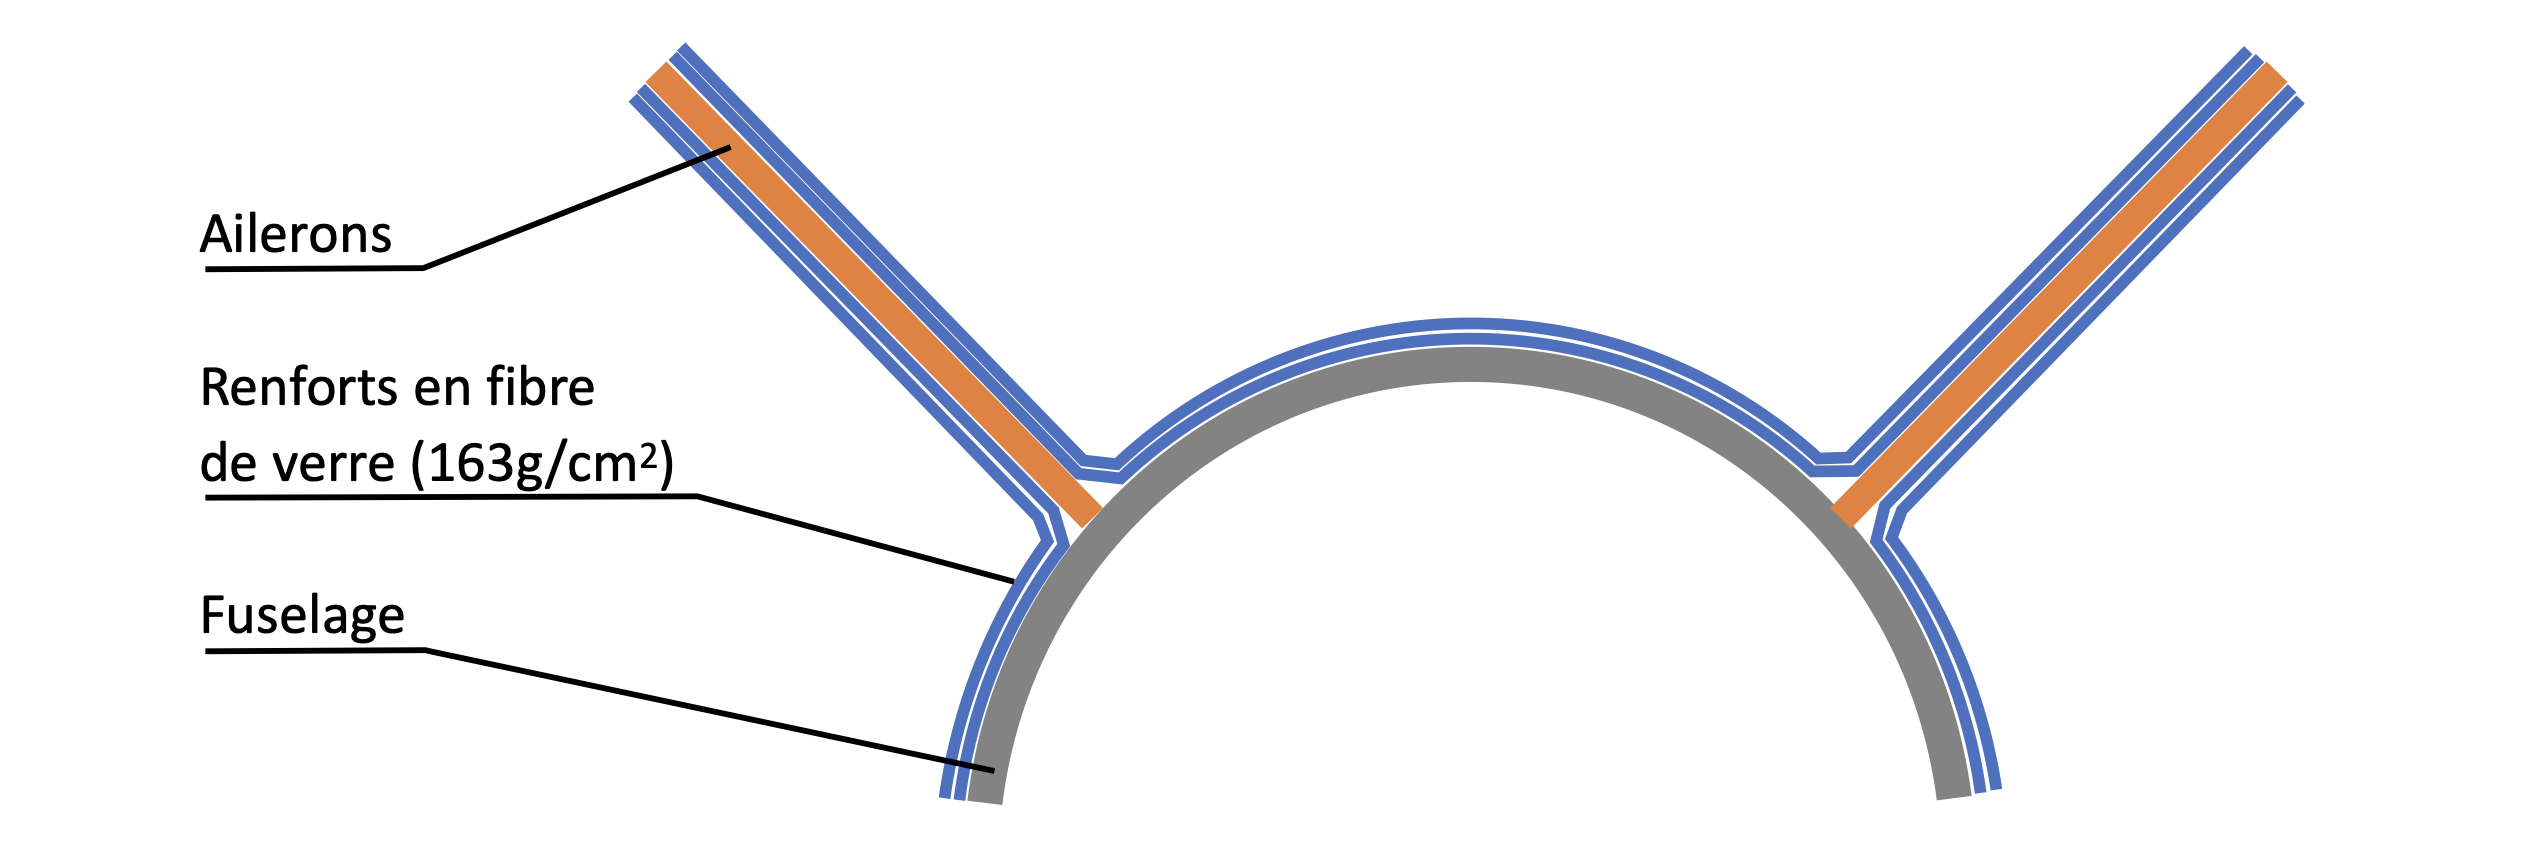
\includegraphics[width=0.8\textwidth]{figures/collage_ailerons_arcturus.png} % Remplacez par le nom de votre fichier image
    \caption{Illustration du collage des ailerons sur le tube de la mini-fusée \textit{Arcturus}.}
    \label{fig:collage_ailerons_arcturus}
\end{figure}



